\documentclass[12pt,a4paper]{article}
\usepackage[utf8]{inputenc}
\usepackage{graphicx}
\parindent0em
\pagestyle{plain}
\usepackage{float}
\begin{document}
	\section{Introduction}
	We implemented the two methods and do not know of any unsolved issues. Everything works as expected. The first method is sp\_exact\_3 which handles exactly 3 sequences. The second method is sp\_approx which can approximate an optimal alignment for multiple sequences.

	\section{Methods}
	Invoke the java files sp\_exact\_3 or sp\_approx to run the algorithms. The algorithms take the first commandline argument as name of the sequence file, if no argument is given they choose "seq.fasta" as default. The solution is written to the file "solution.fasta". (Make sure that "score.txt" is in the same directory).
	\\
	The exact 3 algorithm is implemented by creating a 3-dimensional matrix where we computed the optimal score of the 3 sequences. At each iteration, we compute up to 7 different values, and we choose the minimum of all. After we have finished with the matrix, we have the optimal score on its last cell. Knowing that, we do a backtracking from that point towards the beginning of the sequence and we check where did that value come from and put the result into the alignment strings. We verified that score of the alignment is the same as it is in the \textit{testdata\_short.txt} and \textit{testdata\_long.txt} by checking each result with \textit{msa\_sp\_score\_3k.py}.
	\\
	The approximation algorithm is implemented as in the slides by a method "doAll" and calls "calculateAllPairAlignments" (use solution of the earlier projects), "determineMinimalMiddle" and "extendAlignment". We verified that it is coming close to the optimal solutions.

	\section{Experiments}

	The score of an optimal alignment of the first 3 sequences is 790 and it would look something like:
	\\
	\textgreater brca1\_bos\_taurus (center sequence)
	\\
ATGGATTTATCTGCGGATCATGTTGAAGAAGTACAAAATGTCCTCAATGCTATGCA-GAAAATCTTAG--AGTGTCCAAT-ATGTCTGGAGTTGATCAAAGAG-CCT-GTCTCTACAAAGTGTGA-CCA-CATAT-TTTGCAAATTTTG-TATGCTGAA-AC-TTCTCAACCA-GAAGAAAGGGCCTTCACAATGTCC--TTTGTGTAAGAATGA-
\textgreater brca1\_canis\_lupus
\\
ATGGATTTATCTGCGGATCGTGTTGAAGAAGTACAAAATGTTCTTAATGCTATGCA-GAAAATCTTAG--AGTGTCCAAT-ATGTCTGGAGTTGATCAAAGAG-CCT-GTTTCTACAAAGTGTGA-TCA-CATAT-TTTGCAAATTTTG-TATGCTGAA-AC-TTCTCAACCA-GAGGAAGGGGCCTTCACAGTGTCC--TTTGTGTAAGAACGA-
\textgreater brca1\_gallus\_gallus
\\
GCGAA---ATGTA-ACA-CG-GTAGAGGTGAT-CGGGGTG-CGTT-ATAC-GTGCGTGGTGACCTCGGTCGGTGT-TGACGGTGCCTGGGGTTCCTCAGAGTGTTTTGGGGTCTGAAGGATG-GACTTGTCA-GTGATTGCCATTGGAGACGTGCAAAATGTGCTTTCAGCCATGCAGAA-GAA-CTT-GGAGTGTCCAGTCTGTTTAGATGTGAT
\\
	The score of the first 5 sequences is 3310 and bos\_taurus is the center string.
	\\
	\begin{figure}[h]
  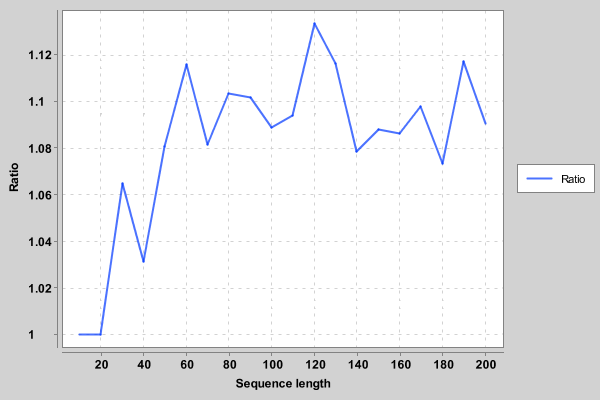
\includegraphics[width=\linewidth]{plotRatio.png}
  \caption{Plot ration sp\_approx/sp\_exact\_3}
  \label{fig:microservQuestion}
\end{figure}
\\
When experimenting with the 20 fasta files (testseqs\_10\_3.fasta, testseqs\_20\_3.fasta, ..., testseqs\_200\_3.fasta) we have observed that there is no difference for the first 2 alignments since their length was small. Overall, the difference in score between the algorithms is increasing but with a small fluctuation. Also, we can notice that as the sequences increase in length, the ratio between these 2 algorithms tends to reach 2(k-1)/k for k sequences. i.e 4/3 in our case, but it never reaches for these given lengths.
	\end{document}